\documentclass{article}
\usepackage{listings}
\usepackage{mathrsfs}
\usepackage[utf8]{inputenc}
\usepackage{amssymb}
\usepackage{lipsum}
\usepackage{amsmath}
\usepackage{fancyhdr}
\usepackage{geometry}
\usepackage{scrextend}
\usepackage[english,german]{babel}
\usepackage{titling}
\usepackage{verbatim}
\setlength{\droptitle}{-3cm}
\usepackage{tikz}
\usepackage{algorithm,algpseudocode}
\usepackage[doublespacing]{setspace}
\usetikzlibrary{datavisualization}
\usetikzlibrary{datavisualization.formats.functions}
\usepackage{polynom}
\usepackage{amsmath}
\usepackage{gauss}
\usepackage{euscript}
\usepackage{tkz-euclide}
\usepackage{stackengine}
\usetikzlibrary{datavisualization}
\usetikzlibrary{datavisualization.formats.functions}
\title{Übungsblatt 5}
\author{
Alexander Mattick Kennung: qi69dube\\
Kapitel 1
}
\usepackage{import}
\date{\today}
\geometry{a4paper, margin=2cm}
\usepackage{stackengine}
\parskip 1em
\newcommand\stackequal[2]{%
  \mathrel{\stackunder[2pt]{\stackon[4pt]{=}{$\scriptscriptstyle#1$}}{%
  $\scriptscriptstyle#2$}}
 }
\makeatletter
\renewcommand*\env@matrix[1][*\c@MaxMatrixCols c]{%
  \hskip -\arraycolsep
  \let\@ifnextchar\new@ifnextchar
  \array{#1}}
\makeatother
\lstset{
  language=haskell,
}
\lstnewenvironment{code}{\lstset{language=Haskell,basicstyle=\small}}{}
\usepackage{enumitem}
\setlist{nosep}
\usepackage{titlesec}
\newcommand{\nto}{\nrightarrow}
\title{Vorlesung 2}
\titlespacing*{\subsection}{0pt}{2pt}{3pt}
\titlespacing*{\section}{0pt}{0pt}{5pt}
\titlespacing*{\subsubsection}{0pt}{1pt}{2pt}



\begin{document}
	%aaron.strahlberger@posteo.de 
	\maketitle
	\section{Aufgabe 1}
	\subsection{1.}
	Sei R eine Relation auf einem DAG, die transitiv ``ist untergraph'' beschreibt.\\
	Der reflexive Abschluss liefert noch keine Problem, der Symmetrische Abschluss führt jedoch dazu, dass zwei unverbundene Elternknoten verbunden sein müssten, (vgl blau runter, grün hoch).\\
	Blau ist die ursprüngliche Relation, rot der reflexive, blau der Symmetrische abschluss.\\
	Orange ist die fehlende Relation zwischen Knoten.\\
	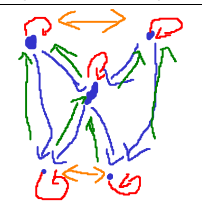
\includegraphics{Relation.png}\\
	\subsection{2.}
	a) R ist transitiv und S ist transitiv $\implies R\cup S$ ist transitiv.\\
	Beweis.:\\
	R ist transitiv: $\forall x,y,z({xRy\land yRz\implies xRz })$\\
	S ist transitiv: $\forall x,y,z({xSy\land ySz\implies xSz })$\\
	die schnittmenge ist daher $\forall x,y,z{(xRy\land yRz\implies xRz )\land (xSy\land ySz\implies xSz )}$ da eine Relation sowohl in R als auch in S gelten muss.\\
	Umformung:\\
	$\forall x,y,z{(xRy\land yRz\implies xRz )\land (xSy\land ySz\implies xSz )}\iff \forall x,y,z{(\lnot(xRy\land yRz)\lor xRz )\land (\lnot(xSy\land ySz)\lor xSz)}$\\
	Distributiv:\\
	$\forall x,y,z ((\lnot(xRy\land yRz)\land\lnot(xSy\land ySz))\lor (\lnot(xRy\land yRz)\land xSz)\lor (xRz\land\lnot(xSy\land ySz))\lor(xRz\land xSz))$\\
	mit de-morgan umformen:\\
	$\forall x,y,z(\lnot ((xRy\land yRz)\lor(xSy\land ySz))\lor \lnot((xRy\land yRz)\lor \lnot xSz)\lor \lnot(\lnot xRz\lor (xSy\land ySz))\lor (xRz\land xSz)$\\
	Nochmal de-morgan:\\
	$\forall x,y,z(\lnot(((xRy\land yRz)\lor (xSy\land ySz))\land((xRy\land yRz)\lor\lnot ySz)\land (\lnot xRz \lor (xSy\land ySz)))\lor (xRz\land xSz) )$\\
	Implikation zurückholen:\\
	$\forall x,y,z (((xRy\land yRz)\lor (xSy\land ySz))\land((xRy\land yRz)\lor\lnot ySz)\land (\lnot xRz \lor (xSy\land ySz)))\implies (xRz\land xSz)) $\\
	Aus unseren Vorraussetzungen wissen wir, dass $xRy\land yRz$ und $xSy\land ySz$ gelten.\\
	Deshalb kann die rechte Seite auf $\top$ reduziert werden.\\
	$\forall x,y,z (\top\land\top\land\top\implies (xRz\land xSz))$\\
	Daraus folgt, dass, wenn R und S transitiv sind, dann auch der Schnitt aus beiden transitiv ist.\\
	b)\\
	Da R symmetrisch ist, gilt $R^-\subseteq R$ ist. Daraus folt die dekomposition von R in $R^-$ und $R$ ist auch teil von R.\\
	Also gilt $R\cup R^-\subseteq R$ (in Worten, eine symmetrische Relation muss mindestens den symmetrischen Abschluss beeinhalten).\\
	Da diese für \textbf{jede beliebige} einzelrelationen in R gilt, kann erweitert werden auf $R\cup R^- = R$, wenn eventuell existierende reflexive einzelrelationen o.b.d.A in beiden R und $R^-$ vorhanden sind.\\
	Das gleiche gilt für S.\\
	also ist $R^-\cup R\cup S\cup S^-= R\cup S$.\\
	Dies kann umgeformt werden in $(R^-\cup S^-)\cup (R\cup S)= R\cup S$.\\
	Was prezise die Vorrausstzung des Symmetrischen abschlusses ist. Daraus folgt unmittelbar: $R\cup S$ ist transitiv.\\
	\subsection{3.}
	a) R ist transitiv und S ist transitiv $\implies R\cup S$ ist transitiv:\\
	Gegenbeispiel: siehe aufgabe 1. (Sei der Transitive abschluss der ursprünglichen blauen R und die grüne symmetrie S).\\
	b) R und s sind transitiv:\\
	Gegenbeispiel: $S=\{(2,2),(1,5)\}$, $R=\{(2,1),(5,2)\}$ führt zu $R\circ S = \{(2,1),(1,2)\}$ Es fehlt $(2,2)$.\\
\end{document}